\documentclass[10pt]{article}
\usepackage[preprint]{tmlr}
\usepackage[hidelinks]{hyperref}
\usepackage{url}
\usepackage{microtype}
\usepackage{amsmath,amssymb,mathtools}
\usepackage{booktabs,tabularx,array,multirow,makecell,threeparttable}
\usepackage{graphicx}
\usepackage{subcaption}
\usepackage{enumitem}
\usepackage{xcolor}
\usepackage{tikz}
\usetikzlibrary{arrows.meta,positioning,calc}
\usepackage[most]{tcolorbox}
\usepackage{caption}
\usepackage{float}
\usepackage[section]{placeins}
\usepackage{nicefrac}

\captionsetup{font=small,labelfont=bf}
\setlist[itemize]{leftmargin=1.5em}
\setlist[enumerate]{leftmargin=1.6em}

\definecolor{fresh}{HTML}{2166AC}
\definecolor{committed}{HTML}{D95F02}
\definecolor{residual}{HTML}{2A9D8F}
\definecolor{softblue}{HTML}{EAF2FB}
\definecolor{softorange}{HTML}{FBE9DD}
\definecolor{softgray}{HTML}{F2F4F7}
\definecolor{softgreen}{HTML}{E7F5F2}
\definecolor{textgray}{HTML}{333333}

\newcommand{\Braw}{B_{\mathrm{raw}}}
\newcommand{\Bcap}{B_{\mathrm{cap}}}
\newcommand{\DeltaBpair}{\Delta B_{\mathrm{pair}}^{\mathrm{cap}}}
\newcommand{\MeanFlip}{\bar{F}}
\newcommand{\DeltaMeanFlip}{\Delta \bar{F}_{\mathrm{pair}}}
\newcommand{\Slead}{S_{\mathrm{lead}}}
\newcommand{\validpair}{\mathrm{valid\_pair\_main}}
\newcommand{\oprefix}{o_{\mathrm{prefix}}}

\title{Revision Barriers in Language Models under Conflicting Evidence}
\author{\name Ali Uyar \\ \addr Independent Researcher}

\begin{document}
\maketitle

\begin{abstract}
Most evaluations measure what a language model currently prefers, not how revisable that preference remains under later conflicting evidence. We introduce a matched-history construction that holds designated incumbent/challenger state and evidence margin fixed while varying the path by which that state was reached. On MHST with Qwen2.5-7B, committed histories are substantially harder to reverse than fresh histories: on held-out paired-valid test pairs, the mean paired barrier gap is 2.78 (95\% CI 2.38--3.19), the leader-consistent subset remains same-sign at 1.85 (1.41--2.30), the required $k{=}0$ cell is exactly null, and an output-margin control stays same-sign. A companion full-curve summary from mean flipability over doses tells the same story. A simple state-only predictor built from designated margin and prefix-only output margin still underpredicts the paired history effect, leaving a positive residual paired gap overall and on the leader-consistent subset. By contrast, a prefix-boundary linear probe does not outperform a prefix-only output-margin baseline overall, and a locked one-site steering test does not yield a qualifying barrier-moving effect, even after a principled boundary-alignment rerun. These results support revision barriers as a behavioral diagnostic of history-sensitive revisability under conflict, while placing clear limits on current latent and causal interpretations.
\end{abstract}

\section{Introduction}

Most evaluations of language models summarize current preference: which answer is leading, which option scores highest, or how large the current evidence margin appears to be. For systems that continue to receive evidence, that is incomplete. Two prefixes can leave a model in the same designated incumbent/challenger support state and with the same designated evidence margin, yet differ systematically in how much later challenger evidence is required to reverse that state. We study that difference as \emph{revisability}.

Our central claim is behavioral rather than mechanistic: matching designated support state is not enough to match revisability. We test this with a matched-history construction that holds the designated incumbent/challenger pair and evidence margin fixed while varying the path by which that state was reached. The resulting asymmetry is summarized by a \emph{revision barrier}: the amount of late challenger evidence needed to flip the incumbent under locked canonical scoring. The main contribution of the paper is to show that this barrier is real and measurable on the primary MHST/Qwen setting, and that it survives a control ladder designed to rule out simpler order-effects readings.

The paper has two main results. The first is a strong behavioral result on MHST/Qwen: committed histories are harder to reverse than fresh histories on held-out test pairs, the leader-consistent subset remains same-sign, the required $k{=}0$ cell is exactly null, and a companion full-curve summary together with an output-margin control tell the same story. The second is a state-only insufficiency result: a simple monotone predictor built from designated margin and prefix-only output margin still underpredicts the paired history effect. These two results are the center of gravity. The latent section is bounded, the one-site causal follow-up is negative under a locked protocol, and the scope evidence is auxiliary.

This is therefore not a paper about anthropomorphic belief states, circuit localization, or a validated causal handle on commitment. We do not claim that the latent probe adds value beyond output margin overall, we do not claim that one-site steering supports causal manipulability of revisability, and we do not claim broad generalization beyond the main MHST/Qwen setting. Instead, we argue for a narrower but substantive conclusion: revision barriers are a useful behavioral diagnostic of history-sensitive revisability under controlled designated state.

\paragraph{Contributions.}
\begin{itemize}
    \item We introduce a matched-history methodology for studying revisability while holding designated incumbent/challenger state and evidence margin fixed.
    \item We establish a strong behavioral revision-barrier result on MHST/Qwen and show that it survives a deliberate control ladder.
    \item We show that a simple state-only predictor built from designated margin and prefix-only output margin still underpredicts the paired history effect.
    \item We document bounded internal follow-ups: a predictive prefix-boundary signal that does not beat output margin overall, and an honest negative one-site steering result.
    \item We report limited auxiliary scope evidence from Llama MHST and RC-ICL without treating those settings as co-equal main results.
\end{itemize}

\section{Matched-history design and evaluation objects}

\subsection{Primary task family: MHST}

We study revisability with \textbf{Matched-History Suspect Tracking} (MHST), a synthetic controlled task designed to separate current designated state from the path that produced it. Each world contains four suspect profiles, each defined by five unique attributes. Prefix clues map unambiguously to one suspect profile. From each base world we generate a \emph{fresh} prefix and a \emph{committed} prefix with the same designated incumbent/challenger pair and the same designated evidence margin $m\in\{1,2,3\}$, but with different evidence order. The history-depth parameter $k\in\{0,1,2\}$ controls how much challenger-consistent prefix evidence is present. After the prefix, a fixed six-slot late packet adds challenger evidence at dose $d\in\{0,\ldots,6\}$.

The primary evaluation uses Qwen2.5-7B-Instruct on held-out MHST test pairs. Auxiliary checks use Llama-3.1-8B on MHST and Qwen2.5-7B on RC-ICL. Those auxiliary settings are reported honestly but are not treated as co-equal main results.

\begin{figure}[t]
    \centering
    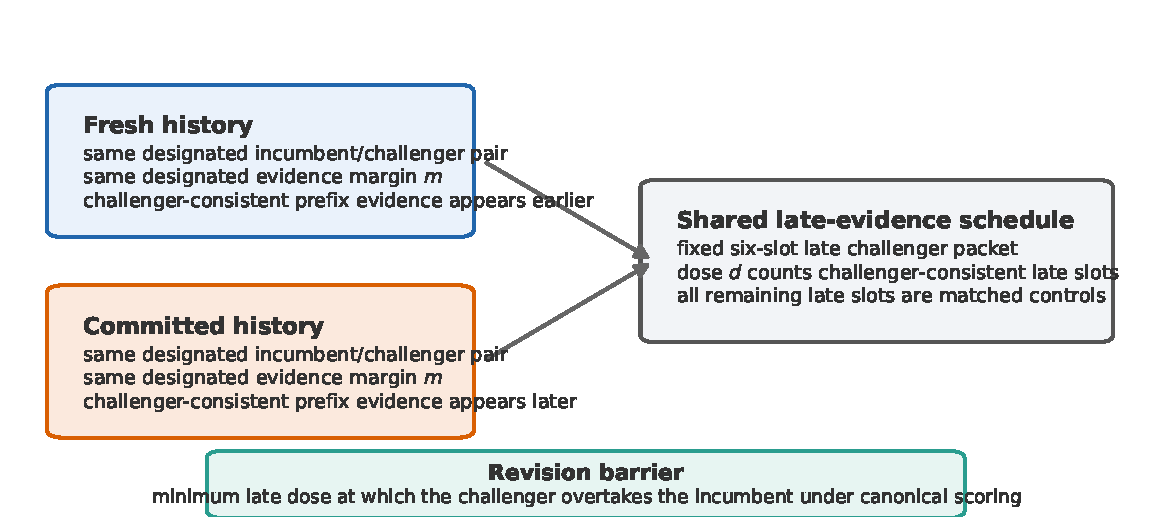
\includegraphics[width=\linewidth]{figures/figure1_matched_history_schematic.pdf}
    \caption{Matched-history construction. Fresh and committed prefixes are matched on the designated incumbent/challenger pair and designated evidence margin, then exposed to the same late challenger-evidence schedule. The behavioral question is whether the same designated state is equally revisable once later counterevidence arrives.}
    \label{fig:matched-history}
\end{figure}

Figure~\ref{fig:matched-history} shows the logic: the paper is about \emph{matching designated state while varying history}. That distinction is critical. The stronger phrase ``same current leader'' is reserved for the leader-consistent subset $\Slead$, defined by prefix-only canonical scoring, and is never used globally.

\subsection{Barrier, reversibility, and paired summaries}

For a prefix $p$, let $q_h(p\oplus U_d)$ denote the canonical score assigned to hypothesis $h$ after appending the late packet $U_d$ at dose $d$. The raw revision barrier is
\begin{equation}
    \Braw(p) = \min\{d\in\{0,\ldots,6\}: q_{\text{challenger}}(p\oplus U_d) \ge q_{\text{incumbent}}(p\oplus U_d)\},
\end{equation}
with $\Braw(p)=\infty$ if no dose flips the ordering. The main scalar summary clips this to
\begin{equation}
    \Bcap(p) = \min(\Braw(p), 7),
\end{equation}
and the paired history effect is
\begin{equation}
    \DeltaBpair(p) = \Bcap(p_{\text{committed}}) - \Bcap(p_{\text{fresh}}).
\end{equation}
Positive values mean that the committed member of a matched pair requires more late challenger evidence to reverse.

We also retain the full reversibility curve
\begin{equation}
    R(d) = \Pr[\Braw \le d],
\end{equation}
and one bounded companion summary based on raw barriers:
\begin{equation}
    \MeanFlip(e) = \frac{1}{7}\sum_{d=0}^{6} \mathbb{1}[\Braw(e) \le d],
\end{equation}
with paired gap $\DeltaMeanFlip = \MeanFlip(\text{fresh}) - \MeanFlip(\text{committed})$.

\subsection{Validity filters and control ladder}

Main behavioral summaries use the paired-valid subset $\validpair$, where neither member of a pair is invalidated by distractor takeover. Stronger same-current-leader wording is reserved for the leader-consistent subset $\Slead$, defined by prefix-only canonical scoring rather than by generation. The behavioral story is further constrained by a required $k{=}0$ null cell, a locked output-margin control, and a no-conflict sanity check that exceeds the project's threshold on MHST/Qwen.

\begin{tcolorbox}[colback=softgreen,colframe=residual!60!black,boxrule=0.8pt,arc=2pt,left=8pt,right=8pt,top=6pt,bottom=6pt]
\textbf{State-only insufficiency proposition.} Consider any account that predicts revisability solely from current-state summaries such as designated margin and prefix-only output margin. In the operational setting of this paper, once designated incumbent/challenger state is matched and those summaries are accounted for, the expected fresh-versus-committed paired gap should vanish. The state-only decomposition in Section~\ref{sec:state-only} tests exactly that implication: the state-only predicted paired gap is the part attributed to current-state summaries alone, and the residual paired gap is the remaining history effect. A positive residual therefore rejects that class of state-only accounts for this matched-history setting.
\end{tcolorbox}

\section{Behavioral revision barriers on MHST/Qwen}
\label{sec:behavior}

The primary result is a strong held-out behavioral asymmetry on MHST/Qwen. On the paired-valid test subset, committed histories require substantially more late challenger evidence to reverse than fresh histories do, with mean $\DeltaBpair = 2.78$ and 95\% CI $[2.38, 3.19]$ across $185$ valid test pairs. The full reversibility curves tell the same story: fresh histories flip earlier and more often than committed histories across the dose schedule (Figure~\ref{fig:main-behavior}A). The paired history-tax distribution is strongly right-shifted rather than being carried by a few extreme outliers (Figure~\ref{fig:main-behavior}B).

\begin{figure}[t]
    \centering
    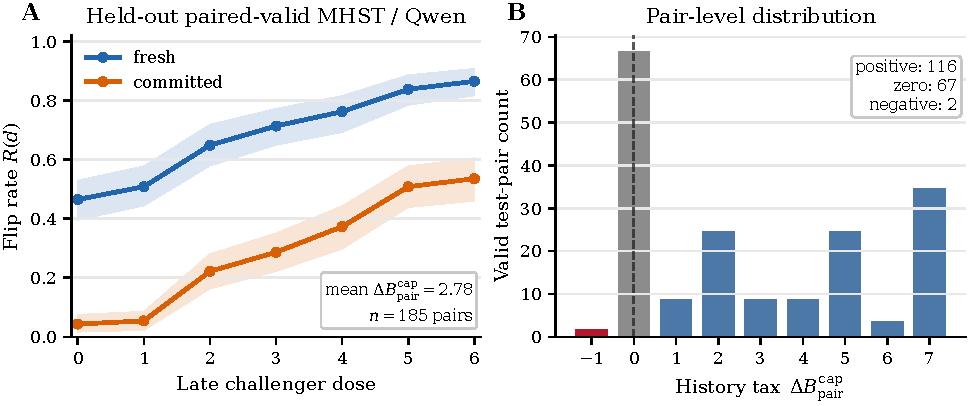
\includegraphics[width=\linewidth]{figures/figure2_main_behavior.pdf}
    \caption{Main behavioral result on held-out MHST/Qwen. \textbf{A}: reversibility curves for fresh and committed histories on the paired-valid test subset, with bootstrap confidence bands. \textbf{B}: distribution of the paired history tax $\DeltaBpair = \Bcap(\text{committed})-\Bcap(\text{fresh})$ over the same valid test pairs. Positive values dominate, showing that committed histories typically require more late challenger evidence to reverse.}
    \label{fig:main-behavior}
\end{figure}

That asymmetry is not uniform noise over the grid. It is structured by $(m,k)$, and the structure is informative. The $k{=}0$ column behaves as an exact null, while the $k{>}0$ cells carry the signal and grow with history depth (Figure~\ref{fig:controls}A). The stronger same-current-leader reading is also supported, but only on the leader-consistent subset: on held-out $\Slead$, the paired-valid mean remains same-sign at $1.85$ with 95\% CI $[1.41, 2.30]$ across $113$ valid pairs. This matters for rhetoric as much as for statistics: it licenses stronger same-current-leader wording locally, but it does not justify using that wording globally.

A separate full-curve summary confirms that the result is not carried only by the clipped barrier scalar. The paired mean-flipability-over-doses gap is $0.3969$ overall (95\% CI $[0.3420, 0.4510]$), remains same-sign on $\Slead$ at $0.2642$ (95\% CI $[0.2035, 0.3300]$), and keeps $k{=}0$ exactly null (Figure~\ref{fig:controls}B). In addition, the locked output-margin control remains same-sign under the required tertile fallback (Appendix~\ref{app:additional-controls}). Taken together, these analyses support a strong behavioral conclusion: matching designated incumbent/challenger state is not enough to determine revisability.

\begin{figure}[t]
    \centering
    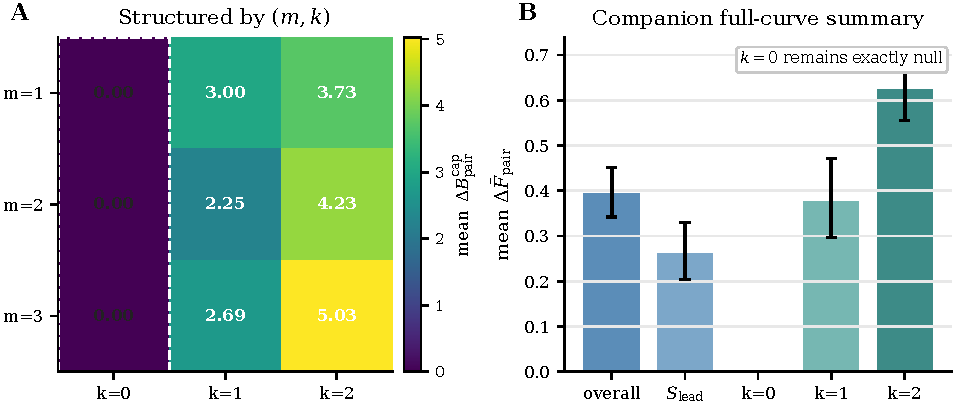
\includegraphics[width=\linewidth]{figures/figure3_control_ladder.pdf}
    \caption{Control ladder for the main MHST/Qwen result. \textbf{A}: mean paired barrier gap by $(m,k)$ on held-out test pairs; the $k{=}0$ column is exactly null, while the $k{>}0$ cells are positive. \textbf{B}: companion full-curve summary from mean flipability over doses. The overall result, the leader-consistent subset, and the $k{>}0$ cells are all same-sign; the $k{=}0$ subset remains exactly null.}
    \label{fig:controls}
\end{figure}

\begin{table}[t]
    \centering
    \small
    \begin{threeparttable}
    \caption{Main behavioral summary on held-out MHST/Qwen test pairs.}
    \label{tab:main-behavior}
    \begin{tabularx}{\linewidth}{>{\raggedright\arraybackslash}X c c c}
        \toprule
        Summary & Pairs & Mean & 95\% CI \\
        \midrule
        Paired barrier gap $\DeltaBpair$ & 185 & 2.7784 & [2.3836, 3.1893] \\
        Leader-consistent paired barrier gap & 113 & 1.8496 & [1.4071, 2.3011] \\
        Companion paired mean-flipability gap $\DeltaMeanFlip$ & 185 & 0.3969 & [0.3420, 0.4510] \\
        Leader-consistent companion gap & 113 & 0.2642 & [0.2035, 0.3300] \\
        \bottomrule
    \end{tabularx}
    \begin{tablenotes}[flushleft]
        \item The required $k{=}0$ cell is exactly null under both summaries. The output-margin control remains same-sign and satisfies the locked control rule under the tertile fallback; the corresponding plot is deferred to Appendix~\ref{app:additional-controls} to keep the behavioral core visually central.
    \end{tablenotes}
    \end{threeparttable}
\end{table}

This control ladder rules out the easiest dismissals without needing more experiments. The result is not simply generic primacy or order sensitivity: the required $k{=}0$ cells remain exactly null, the leader-consistent subset stays same-sign, and the output-margin-controlled analysis stays same-sign. It is also not just a metric trick, because both the clipped barrier summary and the independent full-curve companion summary tell the same story. The paper's main contribution is therefore already established before the internal sections begin.

\section{Current-state summaries are insufficient for revisability}
\label{sec:state-only}

The control ladder in Section~\ref{sec:behavior} already showed that the main MHST/Qwen effect survives several current-state checks: matching of designated incumbent/challenger state by construction, the leader-consistent subset, the exact $k{=}0$ null, and the output-margin control. The state-only insufficiency decomposition compresses that logic into one quantitative object: what a simple current-state model predicts from current-state summaries alone, what the actual paired history effect is, and what residual paired effect remains.

We reuse the same mean-flipability target as the companion behavioral summary. For each valid example $e$, $\MeanFlip(e)$ is the mean over doses of the hard flip indicator derived from raw barriers. We then fit a monotone state-only predictor using only designated margin $m$ and prefix-only output margin $\oprefix$, implemented as isotonic regression of $\MeanFlip$ on $\oprefix$ separately for each $m$ using train examples with valid individual semantics. No history type, $k$, pair identifier, latent feature, or intervention-derived quantity enters the model. The paired prediction is simply the difference between the fresh and committed predictions within each held-out test pair.

The result is clean. On held-out paired-valid test pairs, the observed paired mean-flipability gap is $0.3969$ (95\% CI $[0.3420, 0.4510]$), while the state-only predictor accounts for only $0.3531$ ($[0.3121, 0.3946]$), leaving a positive residual paired gap of $0.0439$ ($[0.0131, 0.0756]$). The same pattern remains on the leader-consistent subset, where the residual is $0.0548$ ($[0.0212, 0.0914]$). The null cell behaves exactly as it should: for $k{=}0$, actual, predicted, and residual gaps are all $0.0$, while the pooled $k{>}0$ subset remains positive with residual $0.0592$ ($[0.0178, 0.1016]$).

\begin{figure}[t]
    \centering
    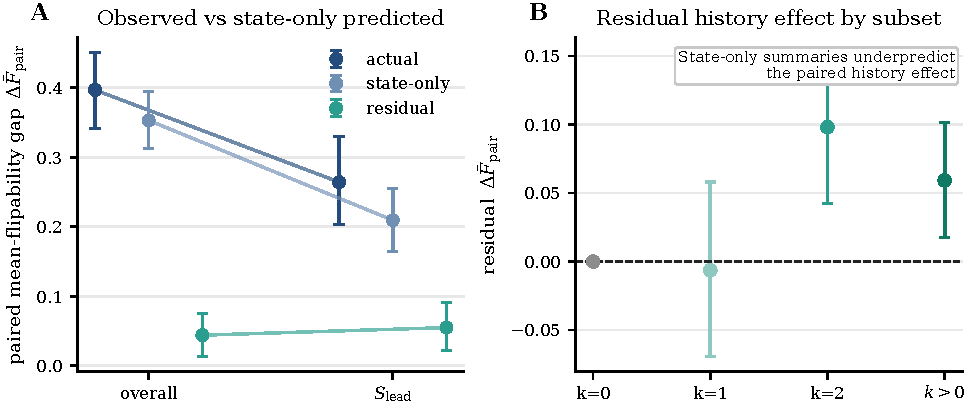
\includegraphics[width=\linewidth]{figures/figure4_state_only_insufficiency.pdf}
    \caption{State-only insufficiency decomposition on held-out MHST/Qwen test pairs. \textbf{A}: actual paired mean-flipability gap, state-only predicted paired gap, and residual paired gap for the overall valid-pair subset and the leader-consistent subset. \textbf{B}: residual paired gap by subset; the $k{=}0$ cell remains exactly null, while $k{>}0$ remains positive. The decomposition therefore shows that current-state summaries underpredict the observed paired history effect.}
    \label{fig:state-only}
\end{figure}

\begin{table}[t]
    \centering
    \small
    \begin{threeparttable}
    \caption{State-only insufficiency decomposition on held-out MHST/Qwen test pairs.}
    \label{tab:state-only}
    \begin{tabularx}{\linewidth}{>{\raggedright\arraybackslash}X c c c c}
        \toprule
        Subset & Pairs & Actual $\DeltaMeanFlip$ & Predicted & Residual \\
        \midrule
        Overall & 185 & 0.3969 [0.3420, 0.4510] & 0.3531 [0.3121, 0.3946] & 0.0439 [0.0131, 0.0756] \\
        Leader-consistent $\Slead$ & 113 & 0.2642 [0.2035, 0.3300] & 0.2094 [0.1645, 0.2550] & 0.0548 [0.0212, 0.0914] \\
        $k{=}0$ & 48 & 0.0000 [0.0000, 0.0000] & 0.0000 [0.0000, 0.0000] & 0.0000 [0.0000, 0.0000] \\
        $k{>}0$ & 137 & 0.5360 [0.4744, 0.5975] & 0.4768 [0.4346, 0.5193] & 0.0592 [0.0178, 0.1016] \\
        \bottomrule
    \end{tabularx}
    \begin{tablenotes}[flushleft]
        \item The state-only model is intentionally narrow: isotonic regression of mean flipability on prefix-only output margin, fitted separately for each designated margin $m$. The residual is therefore the paired history effect not explained by these current-state summaries alone.
    \end{tablenotes}
    \end{threeparttable}
\end{table}

This is the paper's second main result. A simple monotone current-state model built from the two most defensible current-state summaries in the project still underpredicts the paired history effect. That does not make the result latent or causal, but it sharpens the behavioral conclusion: state matching is insufficient for revisability.

\section{Limits of internal explanations}

The next two follow-ups are intentionally bounded. Their role is not to rescue the paper with a stronger mechanistic story, but to document how far the current internal explanations do and do not go.

\subsection{Prefix-boundary signal}

The latent follow-up is informative but secondary. On the original M4 run, the selected prefix-boundary linear probe at layer 24 reached held-out AUROC $0.7921$, clearly exceeding the designated-margin baseline $m$ but falling below both the prefix-only output-margin baseline ($0.8701$) and the combined $[m,\oprefix]$ baseline ($0.8689$). A later boundary-alignment rerun sharpened that conclusion rather than rescuing it: the selected layer changed from 24 to 21 and AUROC rose slightly to $0.8046$, but the probe still lost to both $\oprefix$ and $[m,\oprefix]$ overall. The safe interpretation is therefore narrow: prefix-boundary state contains predictive signal for later revisability beyond designated margin $m$, but not beyond output margin overall.

\subsection{One-site causal follow-up}

The causal lane is an honest negative result. Under the locked one-site steering protocol, the original M5 run selected no nonzero alpha and was therefore unsupported by the project's own rule set. A narrow rerun was justified because an audit found a real extraction/scoring boundary mismatch at the intervention site. That rerun fixed the mismatch, changed the selected latent layer from 24 to 21, and left the full scoring semantics unchanged, so it was a real narrow repair rather than a redesign. But the outcome remained unchanged: on both the original run and the boundary-aligned rerun, every dev example in the movable subset remained row-level flat at every tested signed alpha, no nonzero alpha qualified, and the held-out test steering stage was never entered. Under the locked protocol, C4 is therefore unsupported.



\begin{table}[t]
    \centering
    \scriptsize
    \begin{threeparttable}
    \caption{Bounded internal follow-ups. The latent readout is predictive beyond designated margin but not beyond output margin overall; the one-site steering lane remains unsupported under the locked protocol, including after the boundary-alignment rerun.}
    \label{tab:internal-limits}
    \renewcommand{\arraystretch}{1.08}
    \setlength{\tabcolsep}{4pt}
    \begin{tabularx}{\linewidth}{>{\raggedright\arraybackslash}p{0.24\linewidth} c >{\raggedright\arraybackslash}p{0.16\linewidth} >{\raggedright\arraybackslash}p{0.30\linewidth} >{\raggedright\arraybackslash}p{0.17\linewidth}}
        \toprule
        Follow-up & Layer & Key metric & Comparator & Outcome \\
        \midrule
        \makecell[l]{Original\\M4 probe} & 24 & AUROC 0.7921 & \makecell[l]{$\Delta$ vs $\oprefix = -0.0780$;\\$\Delta$ vs $[m,\oprefix] = -0.0768$} & \makecell[l]{Predictive\\beyond $m$ only} \\
        \makecell[l]{Boundary-aligned\\M4 rerun} & 21 & AUROC 0.8046 & \makecell[l]{$\Delta$ vs $\oprefix = -0.0655$;\\$\Delta$ vs $[m,\oprefix] = -0.0643$} & \makecell[l]{Conclusion\\unchanged} \\
        \makecell[l]{Original\\M5 steering} & 24 & \makecell[l]{no nonzero\\alpha selected} & \makecell[l]{all tested dev shifts flat;\\side effects negligible} & Unsupported \\
        \makecell[l]{Boundary-aligned\\M5 rerun} & 21 & \makecell[l]{no nonzero\\alpha selected} & \makecell[l]{rerun remained row-level\\flat on dev} & Unsupported \\
        \bottomrule
    \end{tabularx}
    \end{threeparttable}
\end{table}

These negative or limited internal results do not make the paper incomplete. They do something more useful: they show that the behavioral effect currently outruns the available internal explanation. This is why the internal material belongs here as a trust-building limits section rather than as a rescue lane.

\section{Auxiliary scope evidence and discussion}

Auxiliary scope evidence is limited but not empty. On Llama-3.1-8B, the MHST effect remained same-sign on held-out test with mean $\DeltaBpair = 0.9231$ and 95\% CI $[0.5897, 1.2827]$, although coverage was much lower than in the primary Qwen run. RC-ICL was also same-sign on its main barrier summaries ($0.5244$, 95\% CI $[0.2043, 0.8401]$) and kept $k{=}0$ exactly null, but it failed its no-conflict cleanliness threshold badly, reaching only $0.70$ where the locked criterion required $0.95$. The safe conclusion is therefore conservative: the effect is not obviously unique to one exact MHST/model configuration, but we do not claim broad generalization beyond the main MHST/Qwen setting. Appendix~\ref{app:scope} gives the corresponding auxiliary curves and summary table.

The paper's main contribution is behavioral and methodological. The matched-history revision-barrier construction gives a concrete way to separate revisability from current designated support state. In the primary MHST/Qwen setting, it yields a strong, well-controlled asymmetry: committed histories are harder to reverse than fresh histories even when the designated incumbent/challenger state and evidence margin are matched by construction. The state-only insufficiency decomposition sharpens that point further: even a simple monotone predictor built from designated margin and prefix-only output margin leaves a positive residual paired history effect.

The internal sections then mark the current interpretive limits. Prefix-boundary state contains signal related to later revisability, but not enough to justify a stronger latent-state claim over output margin. One-site steering does not provide a usable causal handle under the locked protocol, including after a principled boundary-alignment rerun. These follow-ups therefore increase trust not by rescuing a stronger mechanism story, but by showing exactly what the current evidence does \emph{not} support.

The main limitations are straightforward. MHST is synthetic and deliberately controlled, so the strongest claim is about revisability under matched designated state rather than about broad real-world generalization. Auxiliary scope evidence remains limited. And the negative causal result closes only the current one-site steering operationalization; it does not show that no stronger causal account could exist. With those caveats in place, the final claim is narrow but substantive: the matched-history revision-barrier construction is a useful behavioral diagnostic for history-sensitive revisability under controlled designated state.


\bibliographystyle{plainnat}
\bibliography{refs}

\appendix
\section{Additional behavioral controls and auxiliary scope}
\label{app:additional-controls}

\begin{figure}[h]
    \centering
    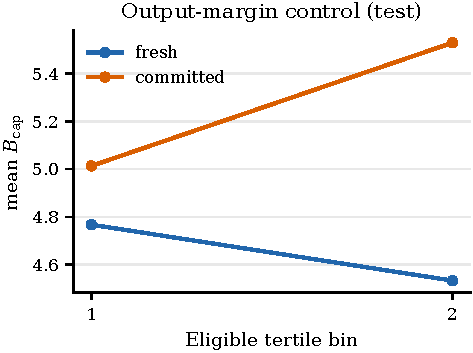
\includegraphics[width=0.58\linewidth]{figures/figureA1_output_margin_control.pdf}
    \caption{Locked output-margin control on held-out MHST/Qwen test pairs. The same-sign effect remains visible under the eligible tertile-bin fallback used by the project.}
    \label{fig:output-margin}
\end{figure}

\begin{table}[h]
    \centering
    \small
    \begin{threeparttable}
    \caption{Auxiliary scope summary. These settings are reported to bound scope, not to carry the paper.}
    \label{tab:scope}
    \begin{tabularx}{\linewidth}{>{\raggedright\arraybackslash}X c c c >{\raggedright\arraybackslash}X}
        \toprule
        Setting & Valid pairs & Mean $\DeltaBpair$ & 95\% CI & Note \\
        \midrule
        MHST / Qwen2.5-7B & 185 & 2.7784 & [2.3836, 3.1893] & Primary setting; no-conflict sanity passes \\
        MHST / Llama-3.1-8B & 39 & 0.9231 & [0.5897, 1.2827] & Same-sign but lower coverage \\
        RC-ICL / Qwen2.5-7B & 225 & 0.5244 & [0.2043, 0.8401] & Same-sign but no-conflict sanity fails ($0.70 < 0.95$) \\
        \bottomrule
    \end{tabularx}
    \end{threeparttable}
\end{table}

\begin{figure}[h]
    \centering
    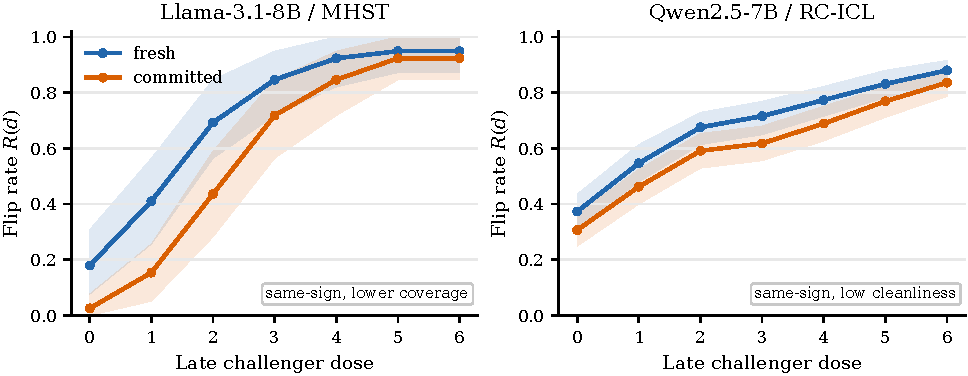
\includegraphics[width=\linewidth]{figures/figureA2_scope_curves.pdf}
    \caption{Auxiliary scope curves. The Llama MHST check is same-sign but lower-coverage. The RC-ICL check is same-sign on its main barrier summary but fails the project's cleanliness threshold, so it remains auxiliary rather than paper-central.}
    \label{app:scope}
\end{figure}


\end{document}
